\documentclass[letterpaper, 10 pt, conference]{../ieeeconf} 
\IEEEoverridecommandlockouts
\overrideIEEEmargins
\pdfoptionpdfminorversion=4

\usepackage{amsmath}
\usepackage{mathtools}
\usepackage{textcomp}
\usepackage{graphicx}
\usepackage[font=footnotesize]{subcaption}
\usepackage[font=footnotesize]{caption}
\usepackage{hyperref}
\usepackage{amssymb}
\usepackage{booktabs}
\usepackage[normalem]{ulem}
\usepackage{verbatim}
\usepackage[export]{adjustbox}
\usepackage{amsmath}
\usepackage{url}
\usepackage{siunitx}
\usepackage[utf8]{inputenc}
\usepackage[TS1,T1]{fontenc}
\usepackage{array, booktabs}
\usepackage{caption}
\usepackage[cal=cm]{mathalfa}
\usepackage{algorithm}
\usepackage[noend]{algpseudocode}

% Labels in IEEE format
\newcommand{\eref}[1]{(\ref{#1})} % Equation
\newcommand{\sref}[1]{Sec.~\ref{#1}} % Section
\newcommand{\figref}[1]{Fig.~\ref{#1}} % Figure
\newcommand{\tref}[1]{Table~\ref{#1}} % Table
\newcommand{\aref}[1]{Algorithm~\ref{#1}} % Algorithm
\newcommand{\lref}[1]{Line~\ref{#1}} % Line
\renewcommand*\rmdefault{ppl}
\setlength{\textfloatsep}{5pt}

\usepackage{ifthen}
\usepackage[usenames,dvipsnames,table]{xcolor}
\newboolean{include-notes}
\setboolean{include-notes}{true} 
% http://en.wikibooks.org/wiki/LaTeX/Colors
\newcommand{\rhnote}[1]{\ifthenelse{\boolean{include-notes}}%
 {\textcolor{blue}{\textbf{RH: #1}}}{}}
\newcommand{\sanote}[1]{\ifthenelse{\boolean{include-notes}}%
 {\textcolor{green}{\textbf{SAN: #1}}}{}}

\begin{document}

% paper title
\title{6.857 Final Project: Milestone 6}
\author{Sebastiani Aguirre Navarro and Rachel Holladay}
\maketitle

% !TEX root = main.tex

\section{Introduction}
\label{sec:intro}

The ability to grasp objects lies at the heart of robotic manipulation and therefore is fundamental to enabling robots to have complex physical interactions with their environment. 
Grasping a variety of unknown objects is challenging due to sensor and actuator uncertainty and uncertainty with respect to a new object's shape, mass distribution, texture properties, etc. 
Recently, deep neural networks have been used, with significant success, to address these challenges and enable robotic grasping. 

Within the context of this paper, we will make three assumptions. 
First, we will be grasping objects from a flat, clutter-free surface, such as an uncrowded table top. 
Second, we assume we have a method of generating \textit{grasp candidates}. 
Last, the robot has either an on-board camera or the environment the robot is operating in has a camera. 
Given an image of the scene captured by the camera, our goal is to evaluate which of these candidate grasps are likely to succeed. 
This creates a binary classification task, where the labels are grasp success and grasp failure. 

During execution, we can imagine that our robot with sample several grasps, execute a grasp that has been predicted to be successful via our classification method.  

For our data set we will use the Dexerity Network (DexNet) 2.0 data set, presented in~\cite{mahler2017dex}. 
The data set has 6.7 million grasps definitions, images and analytical grasp metrics, that we further detailed in \sref{sec:data_set}. 
The authors of the data set trained a Grasp Quality Convolutional Neural Network (GQ-CNN), which achieved 85.7\% accuracy on their classification task.

Using their network, on both our sampled data and their provided data, we were unable to achieve an accuracy rate higher then the percentage of the largest class. We discuss several possible reasons. We then explore several other architectures, with varying hyper parameters and normalization methods. 

\textbf{We make the following contributions}:
\begin{enumerate}
    \item \rhnote{fill in}
		\item \rhnote{fill in}
\end{enumerate}

We first review related work (\sref{sec:related_work}) and further detail the data set (\sref{sec:data_set}). 
Given our data set, we formally define our problem statement (\sref{sec:problem}) and then explore various data sets using the pre-trained GQ-CNN (\sref{sec:balance}). 
We explore other architectures (\sref{sec:archs}) and conclude with a brief discussion (\sref{sec:discussion}). 

\begin{figure}[t!]
    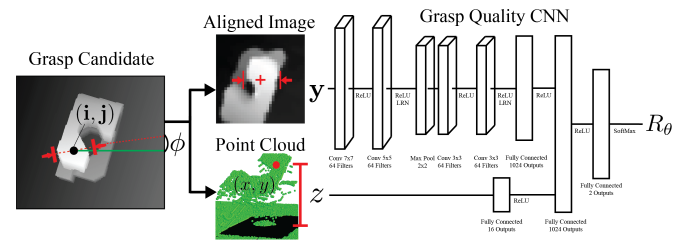
\includegraphics[width=0.99\columnwidth]{figs/dexnet.PNG}
\caption{This is a visualization the GQ-CNN (Grasp Quality Convolutional Neural Network) from \cite{mahler2017dex}. The network takes as input a depth image of the grasp and the distance of gripper to the object and output, after several layers, a prediction of grasp success.} \label{fig:dexnet_network}
\end{figure}

\begin{comment}

To accomplish the same task, we will be experimenting with new architectures, input formats, other modifications described in~\sref{sec:questions}.
Most of the recent machine learning papers in robotics present a problem, dataset and, usually, an optimized convolutional neural network with some architecture and input format. 
Our goal is to explore the process of finding that CNN and exploring the factors that effect performance. 
While our results will only be verified according to this data set, and therefore cannot be generalized to all CNNs, we hope to gain intution, understanding, and, hopefully, a higher accuracy. 
Having explored various components, we will optimize our final, best architecture. 
\end{comment}

% !TEX root = main.tex

\section{Related Work}
\label{sec:related_work}

While we primarily build off of the Dex Net 2.0 paper~\cite{mahler2017dex}, there is a wide range of literature investigating learning how to grasp objects. 
The overwhelming majority of the recent work has focused on using CNNs, although there are a few papers that use SVMs, kernel-density estimation and constrained optimization-based techniques~\cite{jiang2011efficient,kopicki2016one,el2012bridging}. 

Ten Pas et al~\cite{pas2017grasp} developed a grasp detection algorithm similar to the Dex Net paper by generating grasp hypotheses and training a 4-layer CNN to perform binary classification on whether the grasp is viable. 
They use a different grasp representation and rely on the BigBird data set~\cite{singh2014bigbird}. 
Rather then classifying a grasp, Johns et al uses a CNN to learn a grasp function, which provides a score for each grasp~\cite{johns2016deep}. 
At execution time, then can compare the scores of several grasps and select the best grasp.

The above works focus on using a parallel jaw gripper, a two finger hand where the fingers are parallel to each other and usually move together. 
While this is a relatively simple hand, it is ubiquitous in industry and research and still allows for complex manipulation tasks~\cite{mason2011generality}. 
However, people have worked to expand this grasp prediction to more complex, multi-fingered hands using various CNN architectures~\cite{luplanning,varley2015generating,zhou20176dof}. 

Within the grasp learning community, and in fact, within the robotics learning community, there is a pull between real data collected through a robotic platform and data generated from a physics simulator. 
While data collected on a robot better captures reality (since physics simulators are far from perfect), data collection is difficult and time-consuming. 
Pinto et al collected, at the time, a record amount of data at 50k data points of grasps collected across 700 robot hours~\cite{pinto2016supersizing}.
Levine et al later collected 800,000 grasp attempts over a two month period, using between six and fourteen robot arms at once~\cite{levine2016learning}. 
While these approaches allowed them to train a CNN without over fitting or using simulation data, such data collection is not always practical and require a huge amount of engineering effort. 
Bousmalis showed how to augment a smaller amount of real data with simulation to improve accuracy, thus attempting to combine the merits of both~\cite{bousmalis2017using}. 

While most of this work focuses on using color (RGB) or depth (RGBD) images~\cite{lenz2015deep}, there is growing interest in using tactile feedback, inspired by how humans feel as they grasp. 
Calandra et al combines vision and touch sensing to build a visuo-tactile CNN that predicts grasp outcomes from a combination of the modalities~\cite{calandra2017feeling}. 
This can go one step further in using tactile feedback to learn how to readjust while grasping~\cite{chebotar2016self}. 

Dex Net 2.0 is the second of three pieces of research. 
Dex Net 1.0 solves the same grasping problem, but uses a multi-armed bandit model to correlate the rewards of a proposed grasp with previously seen grasps~\cite{mahler2016dex}.
The similarity metric between grasps is learned from a Multi-View CNN. 
Dex Net 3.0 uses a CNN to learn suction points, leveraging recent interest in using suction for pick and place motions~\cite{mahler2017suction}. 

\begin{comment}
BigBird is "a high-quality, large-scale dataset of 3D object instances, with accurate calibration information for every image. We anticipate that “solving” this dataset will effectively remove many perception-related problems for mobile, sensing-based robots."~\cite{singh2014bigbird} 

Grasp detection algorithm for cluttered environments. Generate grasp hypothesis, develop description. Sample a bunch of these and then do binary classification task using a 4-layer CNN. Use big bird~\cite{pas2017grasp}

In this paper, we take the leap of increasing the available training data to 40 times more than prior work, leading to a dataset size of 50K data points collected over 700 hours of robot grasping attempts. This allows us to train a Convolutional Neural Network (CNN) for the task of predicting grasp locations without severe overfitting. In our formulation, we recast the regression problem to an 18-way binary classification over image patches (model grasp-able from different angles)~\cite{pinto2016supersizing}

Detect grasps from RGBD image. Two layer network, early deep learning grasping paper, deals with rgbd instead of just rgb image~\cite{lenz2015deep}. 

grasp proposals from images (not deep learning). focused on novel objects. more descriptive grasp representation, use SVMs \cite{jiang2011efficient}

estimate grasp robustness from local contact patch (use deep learning and random forest)~\cite{seita2016large}

we use dex net 2.0 which builds off of dex net 1.0. This paper presents the Dexterity Network (DexNet) 1.0, a dataset of 3D object models and a sampling-based planning algorithm to explore how Cloud Robotics can be used for robust grasp planning. The algorithm uses a MultiArmed Bandit model with correlated rewards to leverage prior grasps and 3D object models. Dex-Net 1.0 uses Multi-View Convolutional Neural Networks (MV-CNNs), a new deep learning method for 3D object classification, to provide a similarity metric between objects~\cite{mahler2016dex}

present a grasp stability predictor that uses spatio-temporal tactile features collected from the early-object-lifting phase to predict the grasp outcome with a high accuracy. then used to learn grasp readjustments. \cite{chebotar2016self}

action condition video prediction over pixel movement to learn physical interactions, use on a dataset of 59,000 robot interactions involving pushing motions,\cite{finn2016unsupervised}

Deducing whether a particular grasp will be successful from indirect measurements, such as vision, is therefore quite challenging, and direct sensing of contacts through touch sensing provides an appealing avenue toward more successful and consistent robotic grasping. However, in order to fully evaluate the value of touch sensing for grasp outcome prediction, we must understand how touch sensing can influence outcome prediction accuracy when combined with other modalities. Build  visuo-tactile deep neural network models to directly predict grasp outcomes from either modality individually, and from both modalities together. \cite{calandra2017feeling}

learning-based approach to hand-eye coordination for robotic grasping from monocular images. To learn hand-eye coordination for grasping, we trained a large convolutional neural network to predict the probability that taskspace motion of the gripper will result in successful grasps, using only monocular camera images independent of camera calibration or the current robot pose~\cite{levine2016learning}

Dex Net 3.0 uses suction instead, with CNN\cite{mahler2017suction}. 

Hard to collect real robot data. Want to use simulation but simulation doesnt model world precisely. We study how randomized simulated environments and domain adaptation methods can be extended to train a grasping system to grasp novel objects from raw monocular RGB images. (improve accuracy with good simulation and first to use monocular rgb)~\cite{bousmalis2017using}


This paper presents a new method for paralleljaw grasping of isolated objects from depth images, under large gripper pose uncertainty. Whilst most approaches aim to predict the single best grasp pose from an image, our method first predicts a score for every possible grasp pose, which we denote the grasp function. To learn this function, we train a Convolutional Neural Network which takes as input a single depth image of an object, and outputs a score for each grasp pose across the image. Training data for this is generated by use of physics simulation and depth image simulation with 3D object meshes. rhnote{Use same structure as alexnet}~\cite{johns2016deep}

novel approach to multi-fingered grasp planning leveraging learned deep neural network models. We train a convolutional neural network to predict grasp success as a function of both visual information of an object and grasp configuration. We can then formulate grasp planning as inferring the grasp configuration which maximizes the probability of grasp success~\cite{luplanning}

This paper presents a method for one-shot learning of dexterous grasps and grasp generation for novel objects. A model of each grasp type is learned from a single kinesthetic demonstration and several types are taught. These models are used to select and generate grasps for unfamiliar objects. Both the learning and generation stages use an incomplete point cloud from a depth camera. model uses kernel-density estimation. ~\cite{kopicki2016one}

deep learning architecture
for detecting the palm and fingertip positions of stable grasps
directly from partial object views. multi-finger. model is learning grasp quality metrics. Deep Model with local contrast normalization (LCN), 5 convolutional layers, and 3 fully connected layers. experiment with different parameters~\cite{varley2015generating}

s paper considers learning grasps in the full 6D position and orientation pose space for non-parallel-jaw grippers. We generate a database of millions of simulated successful and unsuccessful grasps for a three-fingered underactuated gripper and thousands of objects, and then learn a modified convolutional neural network (CNN) to predict grasp quality from overhead depth images of novel objects.\cite{zhou20176dof}
\end{comment}

% !TEX root = main.tex

\section{Data Set}
\label{sec:data_set}

We opted to use the Dex Net 2.0 data set due to its size, ease of use and parameterization~\cite{mahler2017dex}. 
Large published grasping data sets are rare within robotics, both because the field (data based learning for manipulation) is new and because such data sets are generally difficult to collect. 

Mahler et al define a generative graphical model defined over the camera pose, object shape and pose, friction coefficient, grasp, depth image and success metric. 
To generate the data set they make i.i.d (independent and identically distributed) samples from their generative graphical model, resulting in 6.7 million data points. 

The data set is defined over 1,500 object meshes that were used in Dex-Net 1.0~\cite{mahler2016dex}, collected from a variety of other data bases and standardized with respect to position.
For each object, they generated 100 parallel jaw grasps via rejection sampling of antipodal pairs and evaluated a robust epsilon quality grasp metric on each grasp~\cite{seita2016large}. 
Additionally, each object is paired with a rendered depth image (2.5D point cloud\footnote{The images are 2D matrices that are referred to as 2.5D in robotics literature because they display depth information.}) from the sampled camera pose. 

The data set of 6.7 million data points has 21.1\% positive examples. 
This is unsurprising, since it is much more difficult to find successful grasps, as compared to failed grasps. 

From the data set we randomly sample, with replacement, $k$ data points. 
In some cases we sample such that we guarantee some ratio of positive versus negative examples to explore the effect of varying distributions.  
% !TEX root = main.tex

\section{Problem Statement and Architectures}
\label{sec:problem_and_archs}

\rhnote{Define input and output. Say using cnn. describe software. Describe one-shot learning. then say we investigated the following changes}
\rhnote{Currently, the input format is a 32x32x1 depth map and a 1x7 pose vector. }
\rhnote{For the following results, we use the balanced dataset with our input as the image for each data point and the 7-dimesional grasp vector. 
The data was split into 80\%, 10\% and 10\% for the training, validation and testing sets respectively.}
Use keras ~\cite{chollet2017keras}

\subsection{Balancing Data Sets}
\label{sec:balance}

As mentioned previously, Dex-Net 2.0 contains approximately 20\% positive examples. 

\rhnote{Show what happens if we just use the 80/20 data with confusion matrix. Therefore for the rest of this we used balanced data set. Obviously this limits us because cant use all data set, so We sample}

\subsection{Data Set Size}
\label{sec:size}

\rhnote{To achieve desired ratio mentioned above and for computational reasons, we sample the size of points we use. We can vary this. 10k vs 50k} 

\subsection{Network Structure}
\label{sec:archs}

\rhnote{Describe each of the archs we use. Update this from before}

Andreas Network ~\cite{viereck2017learning}

Below we describe and show the results of two achitectures, which we refer to as the Inception Network~\cite{szegedy2015going} and the ResNet.

The inception network consists of 1 convolution layer in the beginning with 10 filters of size 3x3. 
The output of this layer is passed in parallel to three convolutional layers of sizes 1x1, 3x3, and 5x5, each with 16 filters. 
These outputs are concatenated on the depth dimension and passed through a max pooling layer of 3x3. 
The outputs are flattened with global average pooling and then the pose vector is concatenated before passed to a classifier of one hidden layer of 20 units, as seen in \figref{fig:inception_net}. 

The residual network consists of two convolutional layers, one with 8 filters of size 7x7 and the next with 16 filters of size 3x3.
At this point, the output of this layer branches, such that this same output is passed through two more convolution layers of 32 filters 3x3 and 16 filters 1x1 used as dimension reduction. 
The output of these two layers is added to their input and then passed to another convolution layer of 8 filters of 1x1 for further dimension reduction and then flattened with global average pooling. 
Like for the other network, the pose vector is concatenated to this output before passing it to a classifier with a fully connected layer of 10 hidden units, as shown in \figref{fig:res_net}.

\subsection{Normalization}
\label{sec:normalization}

\rhnote{use l1 and l2 regularization for fully connected layers. use drop out for conv. doesnt make as much sense to use batch normalization because network is not very large}

\section{Results}
\label{sec:results}
Use keras ~\cite{chollet2017keras}
Andreas Network ~\cite{viereck2017learning}

For the following results, we use the balanced dataset with our input as the image for each data point and the 7-dimesional grasp vector. 
During training, 80\% of the dataset was used as train set and the remaining 20\% as test set. 
Below we describe and show the results of two achitectures, which we refer to as the Inception Network~\cite{szegedy2015going} and the ResNet.
As discussed in \sref{sec:questions}, these are the some of the many networks we will be testing.  

The inception network consists of 1 convolution layer in the beginning with 10 filters of size 3x3. 
The output of this layer is passed in parallel to three convolutional layers of sizes 1x1, 3x3, and 5x5, each with 16 filters. 
These outputs are concatenated on the depth dimension and passed through a max pooling layer of 3x3. 
The outputs are flattened with global average pooling and then the pose vector is concatenated before passed to a classifier of one hidden layer of 20 units, as seen in \figref{fig:inception_net}. 

The residual network consists of two convolutional layers, one with 8 filters of size 7x7 and the next with 16 filters of size 3x3.
At this point, the output of this layer branches, such that this same output is passed through two more convolution layers of 32 filters 3x3 and 16 filters 1x1 used as dimension reduction. 
The output of these two layers is added to their input and then passed to another convolution layer of 8 filters of 1x1 for further dimension reduction and then flattened with global average pooling. 
Like for the other network, the pose vector is concatenated to this output before passing it to a classifier with a fully connected layer of 10 hidden units, as shown in \figref{fig:res_net}.
 
In \figref{fig:inception_results}, we can see that for the inception netowrk, the training loss decreases while the validation loss, while oscilating, increases. 
The same trend is shown in \figref{fig:resnet_results} for the residual net. 
This means that, like the results in our previous milestone, the network is overfitting to the data. 
The final training accuracy for inception net and residual net are 70\% and 75\% respectively, while both do 50\% on the validation set. 
One possible modification is to add regularization on the fully connected layers, or to modify the architectures by removing or adding more layers. 
We will continue to explore this as well as experimenting with the representation of the data.

    
\begin{comment}
\begin{figure}[t!]
    \centering
        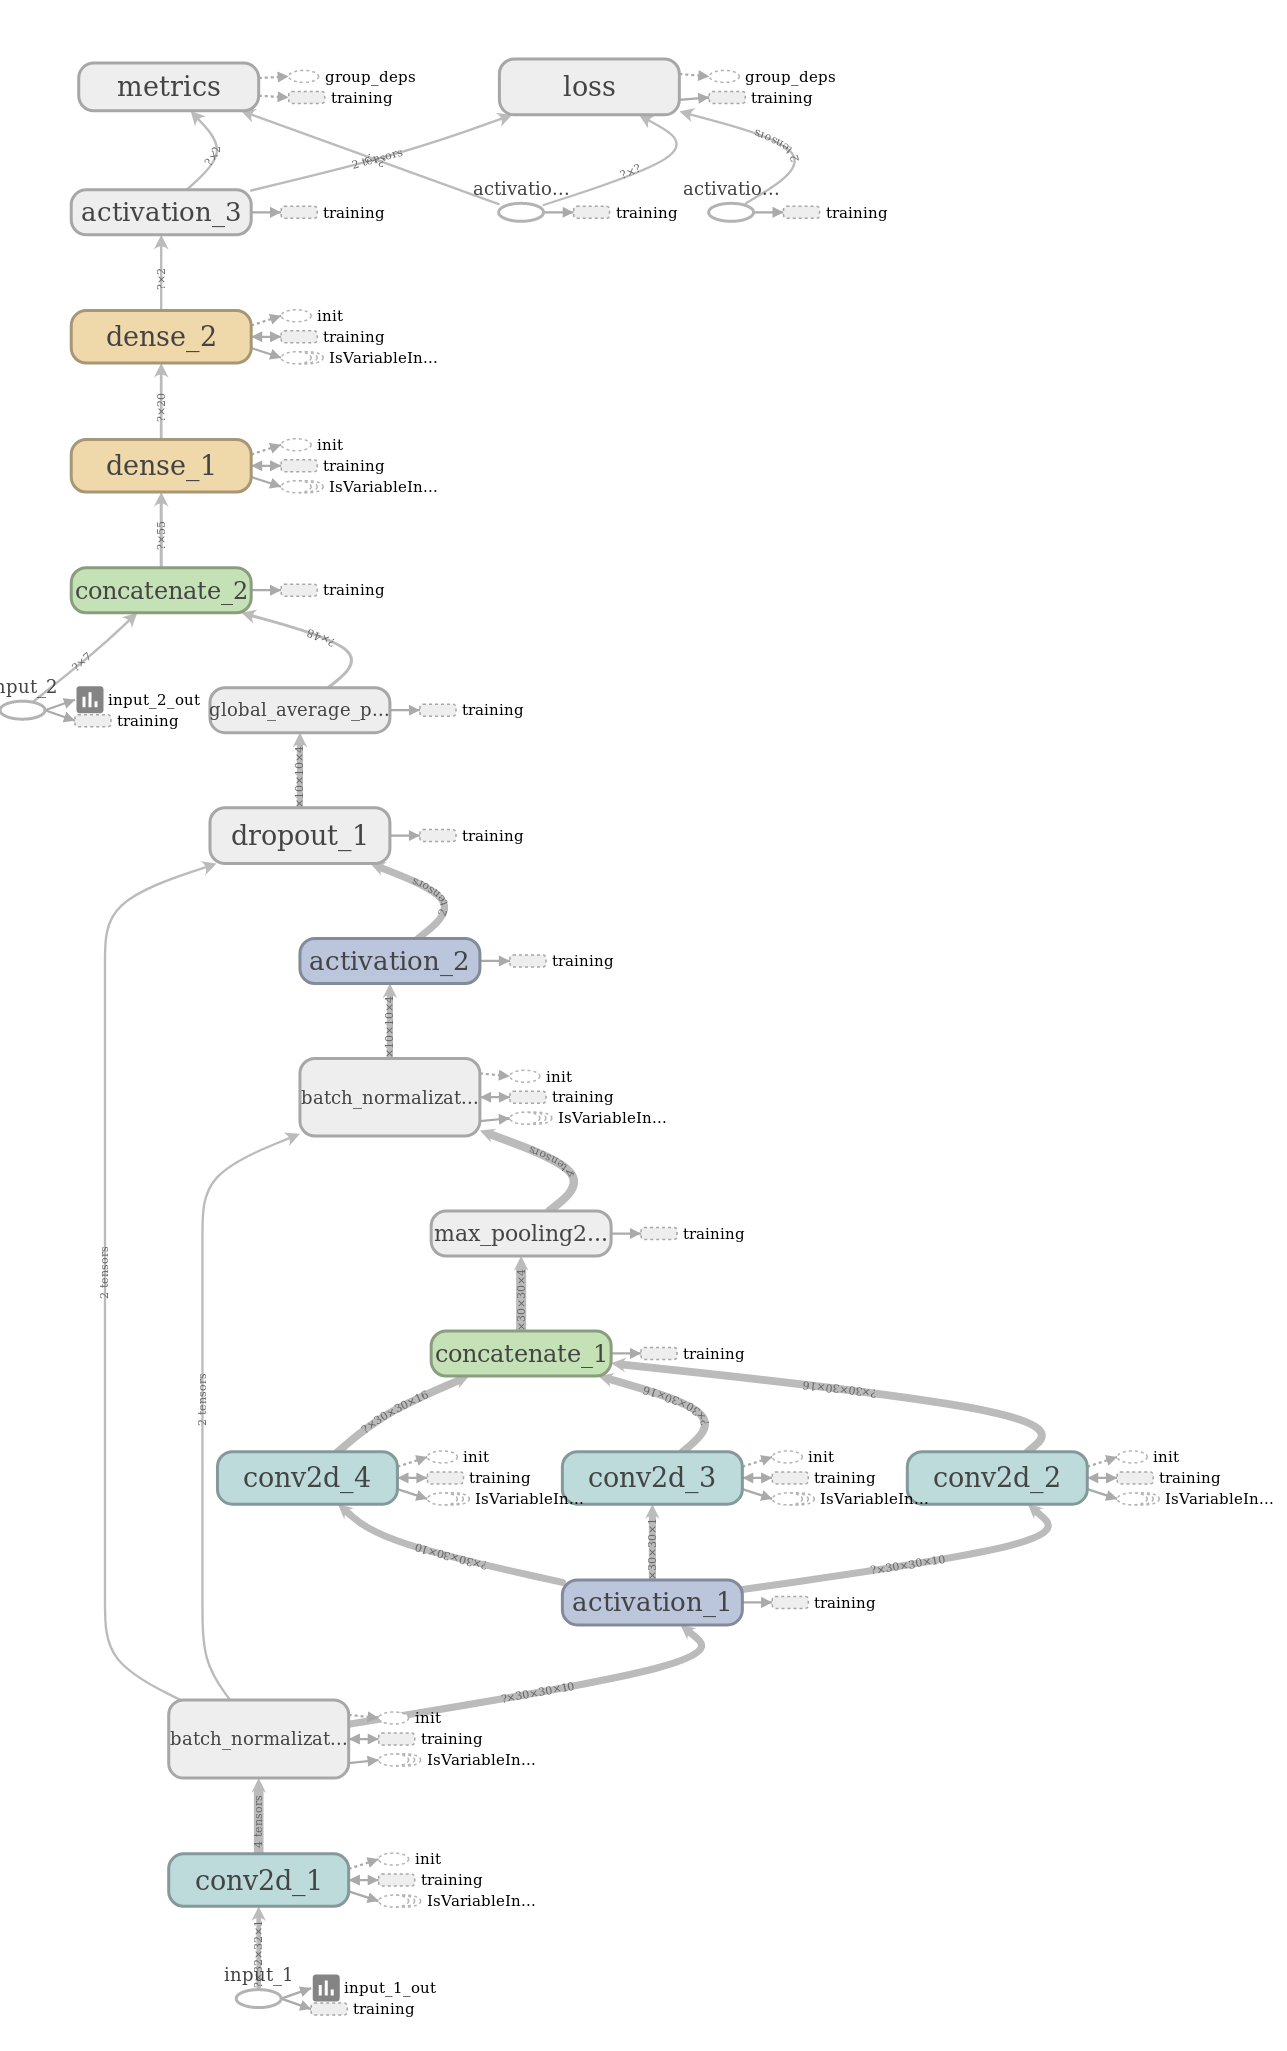
\includegraphics[width=0.7\columnwidth]{figs/inception_net.png}
    \caption{Network Structure of Inception Net} \label{fig:inception_net}
\end{figure}
\end{comment}

{\footnotesize
    \bibliographystyle{ieeetr}
\bibliography{../references}}

\end{document}
